\begin{figure}
	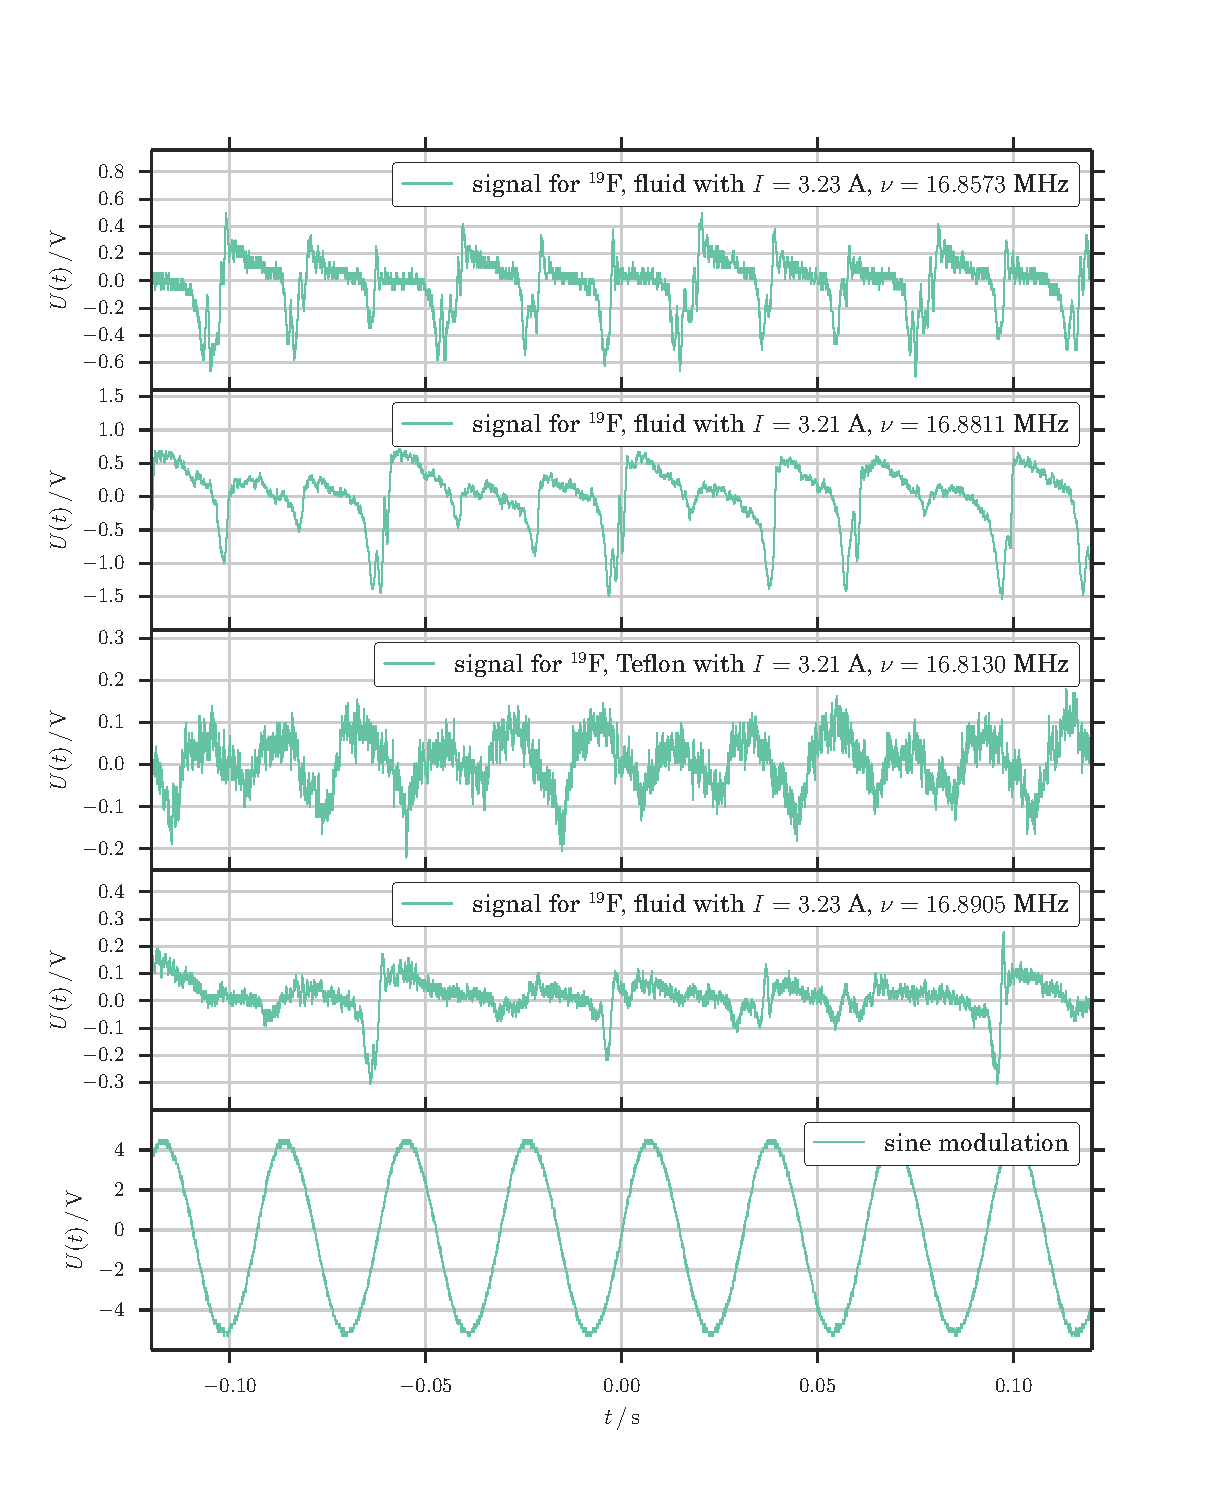
\includegraphics[width=\textwidth]{figures/f_r_F.pdf}
	\caption{
		Absorption peaks of $^{19}$F, measured 
		at four different times. One can observe absorption peaks in each of
		the measured signals. However, due to the described problems with fine tuning,
		we were not able to produce equidistant peaks with a distance of half the,
		wavelength of the input signal, shown in the lowest graph.
		}
	\label{fig:f_r_F}
\end{figure}

\begin{figure}
	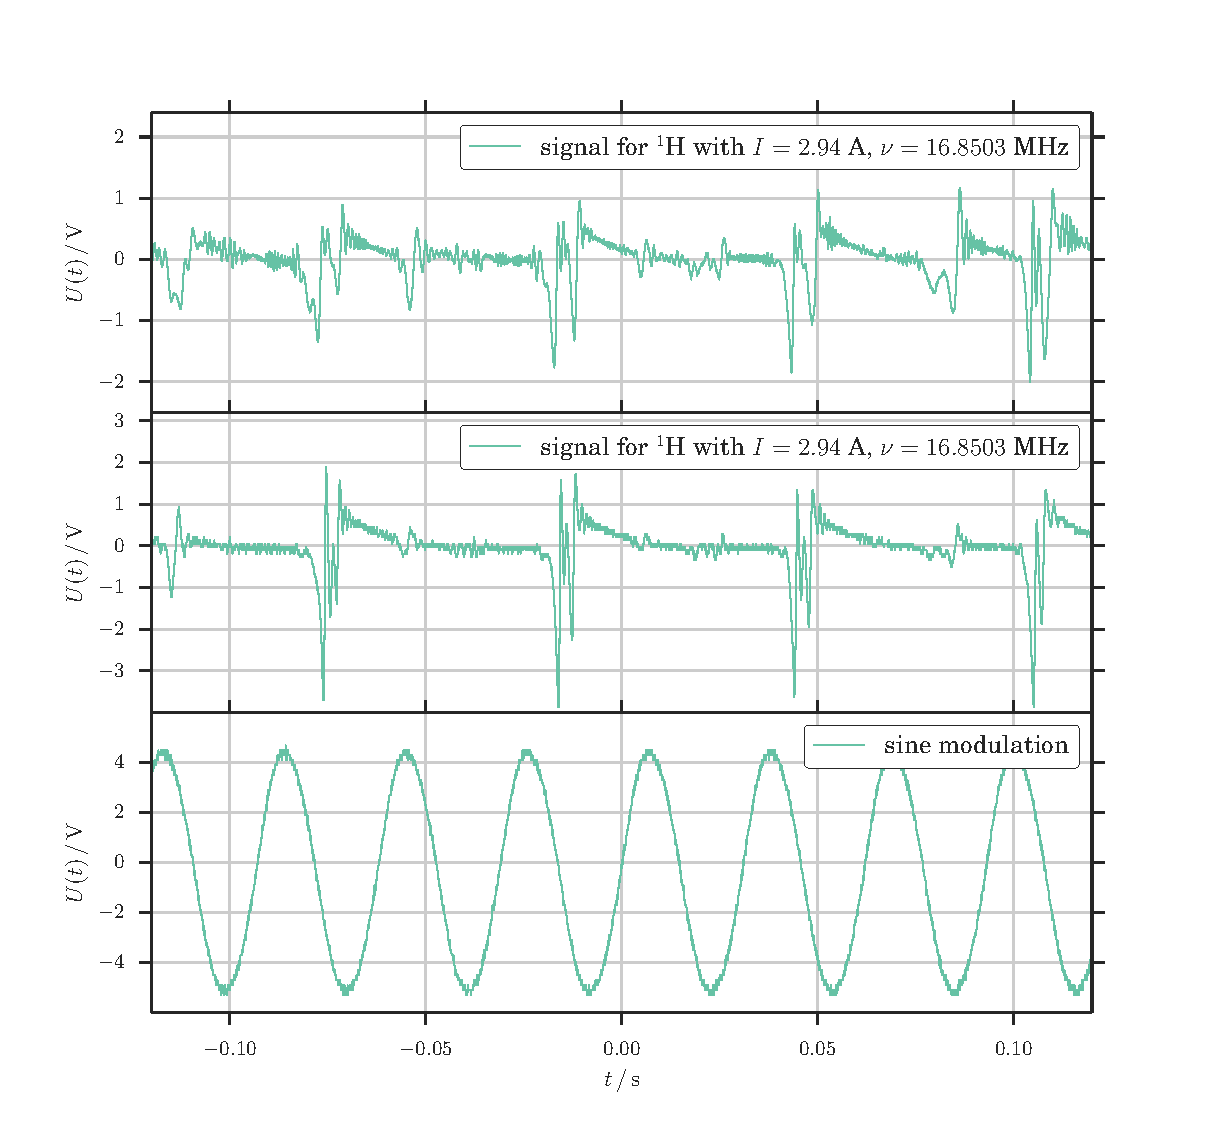
\includegraphics[width=\textwidth]{figures/f_r_H.pdf}
	\caption{
		Absorption peaks of proton ($^1$H) in water
		at two times, both with $B_\mathrm{measured} = 395$ mT.
		No equidistant absorption peaks at the zero intersect of the sine are seen.
		}
	\label{fig:f_r_H}
\end{figure}

\begin{figure}
	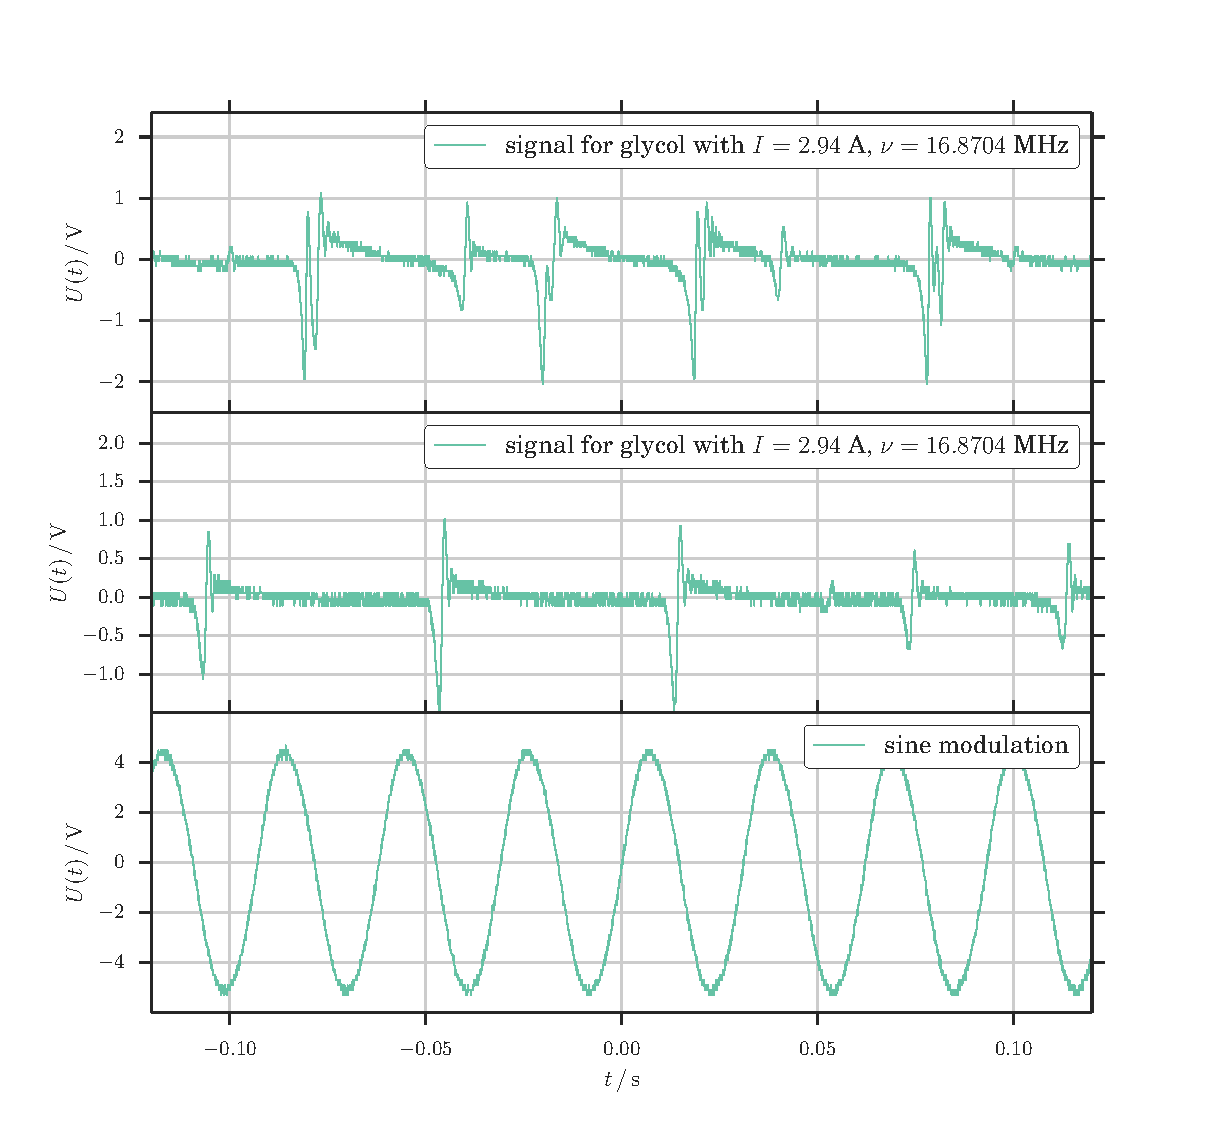
\includegraphics[width=\textwidth]{figures/f_r_glycol.pdf}
	\caption{
		Measured absorption peaks of proton ($^1$H) in glycol
		at two times, both with $B_\mathrm{measured} = 394$ mT.
		Again, no equidistant absorption peaks at the zero intersect of the sine are seen.
		}
	\label{fig:f_r_glycol}
\end{figure}

